%
% Simple asymmetric two-column CV 
% Author: Sofia JIJON
%

\documentclass[a4paper,10pt]{article}
\usepackage[vmargin=.7cm, hmargin=1cm]{geometry}
% !TEX root = Simple-CV.tex
%-------------------------------------------------------------------------------------------------------
% Packages
%-------------------------------------------------------------------------------------------------------
\usepackage[utf8x]{inputenc}
\usepackage[T1]{fontenc}
\usepackage[spanish]{babel}
\usepackage{fontawesome}
\usepackage{datetime}
\usepackage[usenames,dvipsnames]{xcolor}
\usepackage[colorlinks=true, urlcolor=ColorTwo]{hyperref}
\usepackage{tikz}
\usepackage{hyperref}
\usepackage{setspace}
\usepackage{graphicx}
\usepackage{enumitem}
\usepackage{sectsty}
\usepackage{multicol}
\usepackage{adjustbox}
%-------------------------------------------------------------------------------------------------------
% Layout
%-------------------------------------------------------------------------------------------------------
\pagenumbering{gobble}
\renewcommand{\baselinestretch}{1.5} 
\setlength{\parindent}{0pt}

%
% Color theme
%
\definecolor{ColorOne}{RGB}{0,110,140}
\definecolor{ColorTwo}{RGB}{120,0,0}	
\definecolor{ColorThree}{RGB}{50,50,50} 	

%\sectionfont{\color{ColorOne}} 
%\subsectionfont{\color{ColorOne}} 

%
% Vertical line
%
\newcommand{\MyVerticalRule}{
	\textcolor{ColorThree}{\rule{1pt}{\textheight}}
}

%
% Update
%
\newcommand{\LastUpdate}{%
\vfill
\centering \small
\textcolor{ColorOne}{Actualizado: \monthname,~\the\year.}
}

%
% Skip
%
\newcommand{\MySkip}{
\vskip12pt
}

%
% Format hyperrefs
%
\newcommand{\myhref}[2]{%
\href{#1}{\textcolor{ColorThree}{#2}}
}
%
% Format skill bullets
%
\newcommand{\SkillBull}[1]{%
\textcolor{ColorTwo}{#1}
}


%-------------------------------------------------------------------------------------------------------

\begin{document}
\thispagestyle{empty}

%-------------------------------------------------------------------------------------------------------
% Left column
%-------------------------------------------------------------------------------------------------------
\begin{adjustbox}{valign=t}
\begin{minipage}{0.44\textwidth} % Adapt width to your convenience
%----------------------------------------------------
% Please add a photo in 1x1 format
\begin{center}
\begin{tikzpicture}
	\clip (0,0) circle (2cm) node {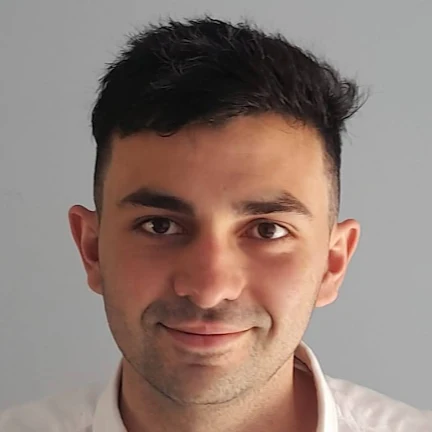
\includegraphics[width=4cm]{foto.png}};
\end{tikzpicture}

\MySkip % See MySetup.tex file

%----------------------------------------------------
{\LARGE \bfseries Renzo Zagarra Saez}

\MySkip % See MySetup.tex file

January 22, 1999\\
Mendoza - Argentina\\

\MySkip %See MySetup.tex file

\textcolor{ColorThree}{\faEnvelopeO} 
\myhref{mailto:renzozagarrasaez@gmail.com}{renzozagarrasaez@gmail.com} \\

\textcolor{ColorThree}{\faGithub} 
\myhref{https://github.com/RenzoZS}{https://github.com/RenzoZS}

\textcolor{ColorThree}{\faLinkedin}
\myhref{https://www.linkedin.com/in/renzo-zagarra-saez-b086311ba/}{Renzo Zagarra Saez}

\end{center}


\section*{About}

I am a physicist, I like to understand things in depth and in the simplest way possible.
I like to share my knowledge and point of view with others, 
and I love to think of the best way to do it. Analytical thinking, mathematics 
and computational skills are my main weapons in problem solving.


\section*{Education}
	\begin{description}
	\raggedright
	
    \item [\normalfont \textcolor{ColorOne}{Aug. 2021 - Dec. 2022.}] \textbf{M.Sc. in Physics}\\
	\href{https://www.ib.edu.ar/}{\textcolor{ColorTwo}{Instituto Balseiro - UnCuyo}}\\
    \textit{Thesis}: Wavefronts in reaction-diffusion equations over heterogeneous media.\\
	

	\item [\normalfont \textcolor{ColorOne}{Aug. 2019 - Dec. 2021.}] \textbf{Bachelor in Physics}\\
	\href{https://www.ib.edu.ar/}{\textcolor{ColorTwo}{Instituto Balseiro - UnCuyo}}\\
    \textit{Thesis}:
    Massively parallel simulations of fire and epidemic propagation models.\;\myhref{https://drive.google.com/file/d/1JmIweLj1CpdmTIp2c9Dv_1kLrm7pwy0D/view?usp=sharing}{\faLink}\\

	\item [\normalfont \textcolor{ColorOne}{Mar. 2017 - Dec. 2018.}] \textbf{Mechatronics Engineering}\\ 
	\href{https://ingenieria.uncuyo.edu.ar/}{\textcolor{ColorTwo}{Facultad de Ingeniería - UnCuyo}}\\
    Two years before applying to Instituto Balseiro.

    \item [\normalfont \textcolor{ColorOne}{Mar. 2012 - Dec. 2016.}] \textbf{Secondary school in Economics and Administration}\\
        \href{https://mzapata.uncuyo.edu.ar/}{\textcolor{ColorTwo}{Escuela de Comercio Martín Zapata - UnCuyo}}\\ 
\end{description}

\vfill
\end{minipage}
\end{adjustbox}
%
%
%-------------------------------------------------------------------------------------------------------
% Vertical rule
%-------------------------------------------------------------------------------------------------------
%
\hfill
\begin{adjustbox}{valign=t}
\begin{minipage}{0.02\textwidth} % Adapt width to your convenience
\MyVerticalRule  % See MySetup.tex file
\end{minipage}
\end{adjustbox}
\hfill
%
%-------------------------------------------------------------------------------------------------------
% Right column
%-------------------------------------------------------------------------------------------------------
\begin{adjustbox}{valign=t}
\begin{minipage}{0.5\textwidth} % Adapt width to your convienience
\section*{Current situation}
\begin{description}
\raggedright
\item[\normalfont \textcolor{ColorOne}{Aug. 2021 -- Dec. 2022.}] \textbf{Master's student}\\ \medskip

\href{https://fisica.cab.cnea.gov.ar/solidos/}{\textcolor{ColorTwo}{Condensed Matter Theory Group}} \\ 
\href{https://fisica.cab.cnea.gov.ar/}{\textcolor{ColorTwo}{Centro Atómico Bariloche}} 
\textcolor{ColorTwo}{-} \href{https://www.argentina.gob.ar/cnea}{\textcolor{ColorTwo}{CNEA}} \textcolor{ColorTwo}{-}
\href{https://www.uncuyo.edu.ar/}{\textcolor{ColorTwo}{UnCuyo}}\\

Development of Python code for solving reaction-diffusion equations with parallel programming techniques using CUDA.

\end{description}
\vspace*{-.6cm}

%----------------------------------------------------
\section*{Experience}
\begin{description}
\raggedright
\item[\normalfont \textcolor{ColorOne}{May. 2021 -- Sep. 2021.}] \textbf{Intern}\\ \medskip
\href{https://fisica.cab.cnea.gov.ar/pop/}{\textcolor{ColorTwo}{Photonics and Optoelectronics Group}}\\	
\href{https://fisica.cab.cnea.gov.ar/}{\textcolor{ColorTwo}{Centro Atómico Bariloche}} 
\textcolor{ColorTwo}{-} \href{https://www.argentina.gob.ar/cnea}{\textcolor{ColorTwo}{CNEA}} \textcolor{ColorTwo}{-}
\href{https://www.uncuyo.edu.ar/}{\textcolor{ColorTwo}{UnCuyo}}\\
Laboratory work with the pump-probe spectroscopic technique and massive experimental data analysis using Python.
    \myhref{https://drive.google.com/file/d/1ekpjBth71yODZ9qb5l38HPsfYHIXj1U6/view?usp=sharing}{\faLink}

\end{description}

\vspace*{-.6cm}
\section*{Skills}
\begin{description}
    \item Software: Python, Wolfram Mathematica, Tex, GitHub, C++, VSCode, Linux, Office
    \item Maths: Modeling, Stochastic Processes, Statistics
    \item Random: Chess, Piano
\end{description}
\vspace*{-.6cm}
\section*{Languages}
\begin{itemize}
	\raggedright
	\item Spanish: Native
	\item English: Intermediate
\end{itemize}

\vspace*{-.6cm}
%----------------------------------------------------
\section*{Presentations}
\begin{description}
	\raggedright
	\item \underline{Renzo Z.}, Alejandro K., \textbf{Propagation of infection/fire fronts on heterogeneous media.} 
    {\href{https://sites.google.com/view/trefemac2022}{\it TREFEMAC}}, May, 2022, La Plata, Argentina. \myhref{https://drive.google.com/file/d/1eik7cwSDLeRaNuslIp8fZdi0H7srbp_F/view?usp=sharing}{\faLink}

\end{description}
\vspace*{-.6cm}
\section*{Courses}
\begin{description}
    \raggedright
    \item \textbf{Data-driven modeling: neural networks, applications and tools.} {\href{https://sites.google.com/view/trefemac2022}{\it TREFEMAC}}, May, 2022, La Plata, Argentina.
    \item \textbf{Mathematical modeling of neural systems} {\href{https://sites.google.com/view/trefemac2022}{\it TREFEMAC}}, May, 2022, La Plata, Argentina.
\end{description}

%----------------------------------------------------


\MySkip
%----------------------------------------------------
%\begin{multicols}{2}
%\section*{Numerical tools}
%\begin{tabular}{ll}
%	R  			& \SkillBull{$\bullet \bullet \bullet \, \circ$}\\
%	Matlab 		& \SkillBull{$\bullet \bullet \bullet \, \circ$}\\
%	Mathematica 	& \SkillBull{$\bullet \circ \circ \, \circ$}\\
%\end{tabular}
%
%\vfill\null \columnbreak  % Break column for new section
%
%\section*{Languages}
%\begin{tabular}{ll}
%	Spanish 		& \SkillBull{$\bullet \bullet \bullet \, \circ$}\\
%	French 		& \SkillBull{$\bullet \circ \circ \, \circ$}\\
%\end{tabular}
%\end{multicols}
%%----------------------------------------------------
\LastUpdate
%%----------------------------------------------------
\end{minipage}

\end{adjustbox}
\end{document}